% -------------------------------- PREAMBLE --------------------------------
\documentclass[a4paper]{report}

\usepackage[utf8]{inputenc}
\usepackage{graphicx}
\usepackage{tikz}
\usepackage{booktabs}
\usepackage[format=hang,font=small,labelfont=bf]{caption}
\usepackage[protrusion=true,expansion=true]{microtype}
\usepackage{amsmath}
\usepackage{amssymb}
\usepackage{amsthm}
\usepackage{upgreek}
\usepackage{nbaseprt}
\usepackage{appendix}
\usepackage{color}
\usepackage{url}
\usepackage{hyperref}
\usepackage{underscore}
\usepackage[numbers]{natbib}
\usepackage{enumitem}
\usepackage{algorithm}
\usepackage{algorithmicx}
\usepackage{algpseudocode}

\newcommand{\reporttitle}{Metric Based Data Analysis Techniques}
\newcommand{\reportauthor}{George Kettleborough}

% --- hyperref stuff ---
\definecolor{darkblue}{rgb}{0,0,0.4}
\hypersetup{
  pdftex,
  bookmarks=true,
  bookmarksopen=true,
  colorlinks=true,
  citecolor=black,
  filecolor=black,
  linkcolor=black,
  urlcolor=darkblue,
  pdfauthor={\reportauthor},
  pdftitle={\reporttitle},
  pdfsubject={}
}
\providecommand{\doi}[1]{\href{http://dx.doi.org/#1}{doi: #1}}

% --- TikZ stuff ---

\usetikzlibrary{calc,trees,positioning,arrows,chains,shapes.geometric,%
  decorations.pathreplacing,decorations.pathmorphing,shapes,%
  matrix,shapes.symbols}

% --- End TikZ stuff ---


% the figures location
\graphicspath{./figures/}

% make equations and figures numbered (sec.eq)
% \numberwithin{equation}{section}
% \numberwithin{figure}{section}

% new operators for maths
\DeclareMathOperator{\op}{op}
\DeclareMathOperator{\remainder}{remainder}
\DeclareMathOperator{\lc}{lc}
\DeclareMathOperator{\pquo}{pquo}
\DeclareMathOperator{\prem}{prem}
\DeclareMathOperator{\pp}{pp}
\DeclareMathOperator{\cont}{cont}
\DeclareMathOperator{\resultant}{resultant}
\DeclareMathOperator{\numerator}{numerator}
\DeclareMathOperator{\denominator}{denominator}
\DeclareMathOperator{\ADCO}{ADCO}
\DeclareMathOperator{\dens}{dens}
\DeclareMathOperator{\symdif}{\bigtriangleup}
\DeclareMathOperator*{\argmin}{arg\,min}
\DeclareMathOperator*{\argmax}{arg\,max}
\DeclareMathOperator*{\tr}{tr}

\newcommand{\dset}{\mathcal{D}}
\newcommand{\clus}{\mathcal{C}}
\newcommand{\NP}{\text{NP}}

% for functions between two partitions C_1 and C_2
\newcommand{\partcompare}[1]{\Delta_{\mathcal{#1}}(\clus_1,\clus_2)}
% for functions between two partitions C and C' and C and C''
\newcommand{\partcomparep}[1]{\Delta_{\mathcal{#1}}(\clus,\clus')}
\newcommand{\partcomparepp}[1]{\Delta_{\mathcal{#1}}(\clus,\clus'')}

% works nicely for fraction indices
\newcommand{\prettyfrac}[2]{^#1\!/\!_#2}

% theorems
\newtheorem{thm}{Theorem}
\newtheorem{lem}{Lemma}
\newtheorem{cor}{Corollary}
\newtheorem{dfn}{Definition}

% problem template
\newenvironment{problem}[1]{\par\addvspace{\topsep}\noindent\textsc{#1}\\}
{\par\addvspace{\topsep}}
\newcommand{\instance}[1]{\textsc{Instance:} #1\\}
\newcommand{\question}[1]{\textsc{Question:} #1}

% algorithmic stuff
\renewcommand{\algorithmicrequire}{\textbf{Input:}}
\renewcommand{\algorithmicensure}{\textbf{Output:}}

\title{\reporttitle}
\author{\reportauthor}

% ------------------------------ END PREAMBLE ------------------------------

\begin{document}

\maketitle

\tableofcontents

\chapter{Introduction}
\label{cha:introduction}

\chapter{Background}
\label{cha:background}

\section{Summary}
\label{sec:summary-backgd}


\section{Datasets and metric spaces}
\label{sec:datas-metr-spac}

A dataset, in the most general terms, is simply a collection of $n$ objects.
Often these objects are $m$-dimensional vectors with each object representing
some observation made during an experiment.  in general, though, we consider
the objects to be of an abstract type about which we know nothing.  For now we
will consider the collection to be a set, but later we will look at some
generalisations.

Let $\dset$ be a dataset and $x,y,z \in \dset$ be objects in the dataset.  If
we wish to learn something about the dataset, one of the first questions we
may ask is, how similar are the objects $x,y$ and $z$?  For this purpose we
have a function $d \colon \dset \times \dset \to \mathbb{R}^+$ where
$d(x,y)>d(x,z)$ means ``$x$ and $y$ are more similar than $x$ and $z$''.  Such
a function is called a \textit{dissimilarity}.

Some dissimilarities are more useful than others.  One would generally expect
such a function to be symmetric, meaning $d(x,y)=d(y,x)$ for all $x,y \in
\dset$.  One would also expect that no two distinct elements can be more
similar than identical elements, so $d(x,x)=0$ for all $x \in \dset$.  A
dissimilarity which satisfies these two properties is called a
\textit{distance}.  When we use a distance, elements are usually said to be
close or distant, instead of similar or dissimilar.

Given a distance, one may also expect that distinct elements are always closer
than identical elements, so $d(x,y)=0$ if \textit{and only if} $x=y$, for all
$x,y \in \dset$.  This is called the identity of indiscernibles.  Further, we
may expect that distances satisfy the triangle inequality, that is
$d(x,y)+d(y,z) \geq d(x,z)$ for all $x,y,z \in \dset$.  A distance which
satisfies these two further requirements is called a \textit{metric}.

Given a set $M$ and a metric $d \colon M \times M \to \mathbb{R}^+$, we call
the ordered pair $(M,d)$ a \textit{metric space}.  If the objects in the
dataset exist in some larger metric space, for example real valued vectors
exist in Euclidean space, then we say the dataset is embedded in a metric
space.

A metric is the most intuitive type of dissimilarity for human use.  Having a
metric allows one to make several deductions quickly and effortlessly.  For
example, if we know that some object $a$ is distant to some other object $b$,
and that a third object $c$ is close to $b$, we would expect that $c$ is also
distant to $a$.  This deduction is correct in a metric space but not correct
in general.

Sometimes when we wish to compare elements of a particular dataset it is
necessary to invent a dissimilarity.  Usually a metric is most desirable.  But
often the objects in the dataset will be of a common type, such as real valued
vectors, for which there are many dissimilarities already defined.  We will
look at some examples of existing dissimilarities now.  Since we are most
interested in metrics, we will only briefly mention some non-metrics.

Dissimilarities which are not distances include Bregman divergences, which are
generalisations of Euclidean distance squared for objects in Euclidean space
\citep{banerjee2005clustering}, and the Kullback-Leibler divergence for
probability distributions \citep{kullback68information}.  Distances which are
not metrics include the Bhattacharyya distance \citep{bhattacharyya43distance}
and in a general positive edge-weighted graph, the length of the shortest path
between two vertices.

We now look at metrics, beginning with Euclidean space.  Let $M$ be
$m$-dimensional Euclidean space and $x=(x_1,x_2,\dotsc,x_m),
y=(y_1,y_2,\dotsc,y_m) \in M$ be any two elements.  Metrics include the
familiar Euclidean distance:
\begin{equation*}
  d_E(x,y) = \sqrt{\sum_{i=1}^{m} (x_i - y_i)^2},
\end{equation*}
the Manhattan distance:
\begin{equation*}
  d_{M}(x,y) = \sum_{i=1}^{m} |x_i - y_i|
\end{equation*}
and the Chebyshev distance:
\begin{equation*}
  d_C(x,y) = \max_{1 \leq i \leq m} |x_i - y_i|,
\end{equation*}
which are all three special cases of the Minkowski distance,
\begin{equation*}
  d_{I}(x,y) = \left(\sum_{i=1}^{m} |x_i - y_i|^{p}\right)^{\prettyfrac{1}{p}}
\end{equation*}
where $p$ is the order; order 1 being Manhattan, 2 Euclidean and $\lim_{p \to
  \inf}$ Chebyshev.

The Mahalanobis distance \citep{mahalanobis30distance} is a metric which is
equivalent to Euclidean distance on scaled principle components of the
dataset.  Given a dataset, $\dset$, of $n$ elements, embedded in
$m$-dimensional Euclidean space, the covariance of components (also known as
features or fields) $i$ and $j$ is defined as
\begin{equation*}
  S_{ij} = \frac{1}{n-1} \sum_{k=1}^{n} (x_{ki}-\bar{x}_i)(x_{kj}-\bar{x}_j),
\end{equation*}
where $x_{ki}$ means the $i$th component of the $k$th element and $\bar{x}_i$
means the mean of component $i$ in the dataset.  The covariance matrix is then
the symmetric $m \times m$ matrix $S = [S_{ij}]$.  The Mahalanobis distance is
then defined as
\begin{equation*}
  d_{P}(x,y) = \sqrt{(x-y)S^{-1}(x-y)^T}.
\end{equation*}

Leaving Euclidean space now, a well known metric on strings of equal length is
the Hamming distance \citep{hamming50errorcodes} which is equal to the number
of positions at which the two strings differ.

For purely categorical data, a simple metric is the overlap metric, or $0/1$
metric:
\begin{equation*}
  d_O(x,y) =
  \begin{cases}
    0 & \text{if $x=y$,} \\
    1 & \text{otherwise.}
  \end{cases}
\end{equation*}

A frequently occurring type of data is mixed data, that is vectors with both
numerical and categorical components.  The heterogeneous Euclidean-overlap
metric uses normalised Euclidean distance on the numerical components and the
overlap metric on categorical components.  It is defined as:
\begin{equation*}
  d_{H}(x,y) = \sqrt{\sum_{i=1}^{m} d_{Hi}^2(x_i,y_i)},
\end{equation*}
where
\begin{equation*}
  d_{Hi}(x_i,y_i) =
  \begin{cases}
    d_O(x_i,y_i) & \text{if $i$ is a categorical component,} \\
    \displaystyle \frac{|x_i-y_i|}{range_i} & \text{otherwise,}
  \end{cases}
\end{equation*}
where $range_i$ is the difference between maximum and minimum observed values
for component $i$.

Metrics are also possible on more complex structures.  Let $S$ be a set of
arbitrary elements and $X,Y \in 2^{S}$ be any two subsets.  The cardinality of
the symmetric difference is a metric on $2^{S}$:
\begin{equation*}
  \delta_{\symdif}(X,Y) = |X \symdif Y|.
\end{equation*}

\begin{figure}
  \centering
  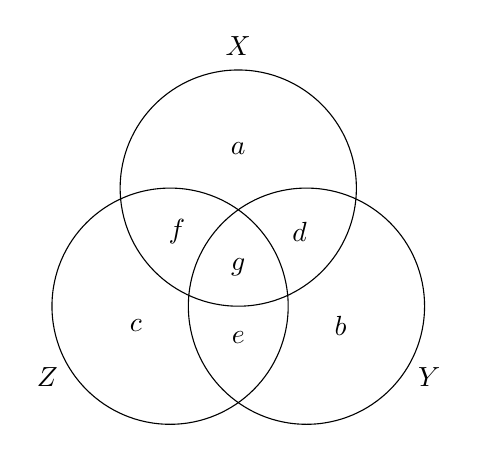
\begin{tikzpicture}
    % circles
    \draw (90:1) circle (1.5);
    \draw (210:1) circle (1.5);
    \draw (330:1) circle (1.5);

    % labels
    \node at (90:2.8) {$X$};
    \node at (330:2.8) {$Y$};
    \node at (210:2.8) {$Z$};
    
    \node at (90:1.5) {$a$};
    \node at (330:1.5) {$b$};
    \node at (210:1.5) {$c$};
    \node at (30:.9) {$d$};
    \node at (270:.9) {$e$};
    \node at (150:.9) {$f$};
    \node at (0:0) {$g$};
  \end{tikzpicture}
  \caption{Partition of $X \cup Y \cup Z$}
  \label{fig:partition}
\end{figure}

\begin{proof}
  It is obvious from the definition that the function is non-negative,
  symmetric and that $\delta_{\symdif}(X,Y)=0$ if and only if $X=Y$ for all
  $X,Y \in 2^{S}$.  We will show that the triangle inequality holds for all
  $X,Y,Z \in 2^{S}$:
  \begin{equation*}
    |X \symdif Y| + |Y \symdif Z| \geq |X \symdif Z|.
  \end{equation*}

  We partition $X \cup Y \cup Z$ into disjoint subsets as shown in
  Figure~\ref{fig:partition} and let
  \begin{align*}
    a &= |A \setminus (B \cup C)|\\
    b &= |B \setminus (A \cup C)|\\
    c &= |C \setminus (A \cup B)|\\
    d &= |(A \cap B) \setminus C|\\
    e &= |(B \cap C) \setminus A|\\
    f &= |(C \cap A) \setminus B|\\
    g &= |A \cap B \cap C|
  \end{align*}

  We can now write the above inequality as:
  \begin{equation*}
    a+2b+c+d+e+2f \geq a+c+d+e,
  \end{equation*}
  so,
  \begin{equation*}
    2b+2f \geq 0.
  \end{equation*}
\end{proof}

The normalised symmetric difference is also a metric on $2^{S}$:
\begin{equation*}
  \delta_{\symdif_n}(X,Y) =
  \begin{cases}
    \displaystyle \frac{|X \symdif Y|}{|X \cup Y|} & \text{if $A \cup B \neq
      \emptyset$} \\
    0 & \text{otherwise.}
  \end{cases}
\end{equation*}

\begin{proof}
  The proof shown here is from \citep{yianilos91}, with some corrections.
  Again, it is easy to see the function is non-negative, symmetric and that
  $\delta_{\symdif_n}(X,Y)=0$ if and only if $X=Y$ for all $X,Y \in 2^{\dset}$
  so we will show that the triangle inequality holds which is:
  \begin{equation*}
    \frac{|X \symdif Y|}{|X \cup Y|} + \frac{|Y \symdif Z|}{|Y \cup Z|} \geq
    \frac{|X \symdif Z|}{|X \cup Y|}
  \end{equation*}
  or, equivalently:
  \begin{equation}
    \label{eq:tri-inequality}
    1 - \frac{|X \cap Y|}{|X \cup Y|} +
    1 - \frac{|Y \cap Z|}{|Y \cup Z|} \geq
    1 - \frac{|X \cap Z|}{|X \cup Z|}.
  \end{equation}

  We partition $X \cup Y \cup Z$ in the same way as in
  Figure~\ref{fig:partition} and with $a,b,c,d,e,f,g$ defined as in the
  previous proof and also we define
  \begin{equation*}
    \xi  = |X \cup Y \cup Z|.
  \end{equation*}

  We can now write equation~(\ref{eq:tri-inequality}) as
  \begin{equation*}
    1 - \frac{d+g}{\xi -c} + 1 - \frac{e+g}{\xi -a} \geq 1 - \frac{f+g}{\xi -b}
  \end{equation*}
  which can be rewritten as
  \begin{equation*}
    \frac{d+g}{\xi -c} + \frac{e+g}{\xi -a} \leq \frac{f+g}{\xi -b} + 1.
  \end{equation*}

  Removing $b$ from the denominators on the LHS can only make the LHS
  greater, so it is sufficient to show that
  \begin{equation*}
    \frac{d+g}{\xi -b-c} + \frac{e+g}{\xi -a-b} \leq \frac{f+g}{\xi -b} + 1.
  \end{equation*}

  Now if we replace $1$ with $\frac{\xi -a-b-c}{\xi -a-b-c}$ on the RHS and add
  the fractions on the LHS we get
  \begin{multline*}
    \frac{(\xi -a-b)(d+g)+(\xi -b-c)(e+g)}{(\xi -b-c)(\xi -a-b)}\\
    \leq \frac{(\xi -a-b-c)(\xi -b)+(\xi -a-b-c)(f+g)}{(\xi -b)(\xi -a-b-c)}
  \end{multline*}
  which when we expand the denominators becomes
  \begin{multline*}
    \frac{(\xi -a-b)(d+g)+(\xi -b-c)(e+g)}{\xi ^2-\xi a-2\xi b-\xi c+ab+bc+b^2+ac}\\
    \leq \frac{(\xi -a-b-c)(\xi -b)+(\xi -a-b-c)(f+g)}{\xi ^2-\xi a-2\xi b-\xi c+ab+bc+b^2}.
  \end{multline*}
  Notice that the denominator on the LHS is equal to the denominator on the
  RHS with the addition of $ac$ so it cannot be less.  It is therefore
  sufficient to show that
  \begin{multline*}
    (\xi -a-b)(d+g)+(\xi -b-c)(e+g)\\
    \leq (\xi -a-b-c)(\xi -b)+(\xi -a-b-c)(f+g).
  \end{multline*}

  Starting with the LHS we have
  \begin{align*}
    &(\xi -a-b)(d+g)+(\xi -c-b)(e+g)\\
    &= (\xi -a-b-c)(d+g)+c(d+g)+(\xi -a-b-c)(e+g)+a(e+g)\\
    &\leq (\xi -a-b-c)(d+g)+c(\xi -a-b-c)\\
    &\qquad\qquad+(\xi -a-b-c)(e+g)+a(\xi -a-b-c)\\
    &= c(\xi -a-b-c)+(\xi -a-b-c)(d+e+g)\\
    &\qquad\qquad+g(\xi -a-b-c)+a(\xi -a-b-c)\\
    &\leq c(\xi -a-b-c)+(\xi -a-b-c)^2+g(\xi -a-b-c)+a(\xi -a-b-c)\\
    &= (\xi -a-b-c)(\xi -b)+g(\xi -a-b-c)\\
    &\leq (\xi -a-b-c)(\xi -b) + (f+g)(\xi -a-b-c).
  \end{align*}
\end{proof}

If the sets are nonempty subsets of a metric space, $(M,d)$ then the
underlying metric space can be used to define metrics on the sets.  The
Haussdorf metric is a metric on $2^{M}$ \citep{braun2003geometry}:
\begin{equation*}
  \delta_{H}(X,Y) = \max(\max_{x \in X} \min_{y \in Y} d(x,y),
                        \max_{y \in Y} \min_{x \in X} d(x,y)).
\end{equation*}
In Chapter~\ref{cha:assignment-metric} we present another metric which can be
used for this purpose.

As an aside, it should be noted that
\begin{equation*}
  \delta(X,Y) = \min_{x \in X, y \in Y} d(x,y)
\end{equation*}
is a simple and intuitive distance between sets, but is not generally a
metric.

Many other metrics exist including the Hellinger distance and Jensen-Shannon
divergence squared \citep{endres03metric} for probability distributions.
There exist generalised Mahalanobis distances for mixed data
\citep{leon2005generalized}.  In Section~\ref{sec:comparing-partitions} we
look at metrics (and general dissimilarities) on partitions and in
Chapter~\ref{cha:assignment-metric} we introduce our own metric.

It is also possible in some cases to transform a general dissimilarity into a
metric, for example see \citet[chap. 2.5]{everitt80}.

It is tempting to think of a dataset and a metric defined on its elements as a
metric space, but this is not necessarily correct.  The reason is that,
contrary to the name, a dataset is not a set but a multiset.  Consider a
dataset consisting of only the heights of some population of humans.
Depending on the precision of the measurements taken, it would generally be
expected that multiple people will share the same height.  In order to have
these observations in a set, some unique integer---an experiment number,
say---would need to be attached to each observation.  But then the metric
condition that $d(x,y)=0$ only if $x=y$ would be violated---in fact we would
have only a pseudometric.  We can get a proper metric if we define an
equivalence relation $x \sim y$ if $d(x,y)=0$.  Then $(\dset/\sim,d)$ is a
metric space.

Most of the time we do not need to worry about this.  From now on a dataset,
$\dset$, will implicitly mean $\dset/\sim$ as defined above unless stated
otherwise.  Occasionally. though, it will be useful or necessary to consider
the multiset $(\dset,\mu_{\dset})$ where $\dset$ is the underlying set, and
$\mu_{\dset} \colon \dset \to \mathbb{N}_1$---a map from $\dset$ to the
(nonzero) natural numbers---is called the membership function and tells us how
many times an element appears in the multiset.

A further generalisation is then possible: we can relax the definition of the
membership function to $\mu_{\dset} \colon \dset \to \mathbb{R}_1$---a map
from $\dset$ to the positive real numbers.  The dataset is then a fuzzy
multiset.  Such datasets have been used in document clustering applications,
for example in \citep{miyamoto2003information}, where objects can appear
multiple times with a certain probability attached.  If the membership
function if $\mu_{\dset} \colon \dset \to \mathbb{R}_1 \cap [0,1]$ then
$(\dset,\mu_{\dset})$ is called a fuzzy set
\citep{zadeh1965fuzzy,gottwald2010fuzzy}.

\section{Partitions}
\label{sec:partitions}

In this section we look at the properties of partitions of datasets, how we
can compare partitions and how we can find partitions.

\subsection{The space of partitions}
\label{sec:space-partitions}

A partition of a dataset, $\dset$, is a set of $k$ sets, $C_1C_2,\dotsc,C_k$
where $C_1 \cup C_2 \cup \dotsb \cup C_k = \dset$, $C_i \neq \emptyset$ for
all $1 \leq i \leq k$ and $C_i \cap C_j = \emptyset$ for all $1 \leq i < j
\leq k$.  In other words, it is a set of nonempty, nonoverlapping subsets.
These subsets are called clusters.

\begin{figure}
  \centering
  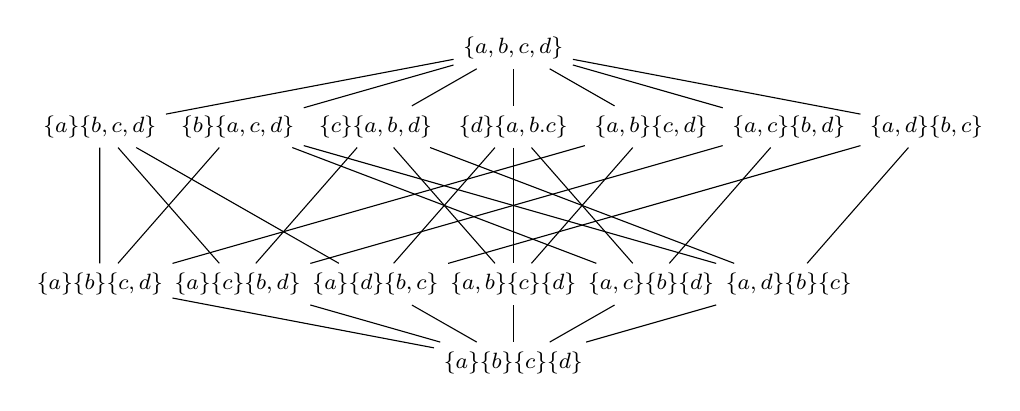
\begin{tikzpicture}[
    xscale=1.75, font=\footnotesize]

    % vertices
    
    \node (0) at (0,0) {$\{a,b,c,d\}$};

    \node (10) at (-3,-1) {$\{a\}\{b,c,d\}$};
    \node (11) at (-2,-1) {$\{b\}\{a,c,d\}$};
    \node (12) at (-1,-1) {$\{c\}\{a,b,d\}$};
    \node (13) at (0,-1) {$\{d\}\{a,b.c\}$};
    \node (14) at (1,-1) {$\{a,b\}\{c,d\}$};
    \node (15) at (2,-1) {$\{a,c\}\{b,d\}$};
    \node (16) at (3,-1) {$\{a,d\}\{b,c\}$};

    \node (20) at (-3,-3) {$\{a\}\{b\}\{c,d\}$};
    \node (21) at (-2,-3) {$\{a\}\{c\}\{b,d\}$};
    \node (22) at (-1,-3) {$\{a\}\{d\}\{b,c\}$};
    \node (23) at (0,-3) {$\{a,b\}\{c\}\{d\}$};
    \node (24) at (1,-3) {$\{a,c\}\{b\}\{d\}$};
    \node (25) at (2,-3) {$\{a,d\}\{b\}\{c\}$};

    \node (3) at (0,-4) {$\{a\}\{b\}\{c\}\{d\}$};

    % edges

    \draw (0) to (10);
    \draw (0) to (11);
    \draw (0) to (12);
    \draw (0) to (13);
    \draw (0) to (14);
    \draw (0) to (15);
    \draw (0) to (16);

    \draw (10) to (20);
    \draw (10) to (21);
    \draw (10) to (22);
    \draw (11) to (20);
    \draw (11) to (24);
    \draw (11) to (25);
    \draw (12) to (21);
    \draw (12) to (23);
    \draw (12) to (25);
    \draw (13) to (22);
    \draw (13) to (23);
    \draw (13) to (24);
    \draw (14) to (20);
    \draw (14) to (23);
    \draw (15) to (21);
    \draw (15) to (24);
    \draw (16) to (22);
    \draw (16) to (25);

    \draw (20) to (3);
    \draw (21) to (3);
    \draw (22) to (3);
    \draw (23) to (3);
    \draw (24) to (3);
    \draw (25) to (3);
  \end{tikzpicture}
  \caption{The lattice of partitions of dataset $\{a,b,c,d\}$ \citep{meila-2005}.}
  \label{fig:lattice}
\end{figure}

\begin{table}
  \centering
  \begin{tabular}{rr}
    \toprule
    $n$ & $B_n$ \\
    \midrule
    5 & 52 \\
    10 & 115,975 \\
    15 & 1,382,958,545 \\
    20 & $5.17 \times 10^{13}$ \\
    25 & $4.64 \times 10^{18}$ \\
    \bottomrule
  \end{tabular}
  \caption{Growth of the Bell number}
  \label{tab:bell-number}
\end{table}

Let $\mathcal{P}_{\dset}$ be the set of all partitions of $\dset$.  The
natural way to represent the set $\mathcal{P}_{\dset}$ is as a graph called
the lattice of partitions.  Such a graph is shown in Figure~\ref{fig:lattice}.
The top of the graph contains a single node containing $\hat{1} = \{\dset\}$
which is the partition with one cluster and the bottom is a single node
containing $\hat{0} = \{\{D_1\},\{D_2\},\dotsc,\{D_n\}\}$ the partition
containing $n$ clusters.

A partition, $\clus'$, which is obtained by splitting one or more clusters in
$\clus$ is said to be a refinement of $\clus$.  Every edge in the lattice
represents a refinement, with the coarser partition at the top.

As can be seen from Figure~\ref{fig:lattice}, the number of possible
partitions for a 4 element dataset is already quite large; for a 20 element
dataset the number is more than 51 trillion.  In general the number of
possible partitions of an $n$ element dataset is equivalent to the $n$th Bell
number, $B_n$~\citep{bell1934exponential}.  The sequence of Bell numbers
begins with $B_0 = 1$ and its growth is then superexponential in $n$.  The
rest of sequence can be generated in a few ways including by a recursive
formula:
\begin{equation*}
  B_n = \sum_{k=0}^{n-1} B_k {n-1 \choose k},
\end{equation*}
or using Dobinski's formula:
\begin{equation*}
  B_n = \frac{1}{e} \sum_{k=0}^{\inf} \frac{k^n}{k!}.
\end{equation*}

Partitions can be generalised to fuzzy partitions by allowing elements to be
in more than one cluster.  A fuzzy partition is therefore a set of fuzzy sets
$\{(C_i,\mu_i),(C_2,\mu_2),\dotsc,(C_k,\mu_k)\}$ where $C_1 \cup C_2 \cup
\dotsb \cup C_k = \dset$, $C_i \neq \emptyset$ for all $1 \leq i \leq k$ and
$\sum_{i=1}^{k} \mu_i(x) = 1$ for all $x \in \dset$.

\subsection{Comparing partitions}
\label{sec:comparing-partitions}

An attractive way to find partitions of a dataset is by means of a partitional
clustering method.  Many methods exist---we will review some in
Section~\ref{sec:part-clust-algor}---and each method tends to produce
a different partition.  Some methods are non-deterministic and produce
different partitions each time.

It is therefore useful, for comparing and assessing clustering methods, to be
able to compare partitions.  Such a comparison measure is also used in
ensemble clustering, where multiple methods are used and partitions are voted
on.  Many measures have been devised for this purpose, including similarity
measures and dissimilarity measures, of which some are metrics.  Existing
methods fall into four main categories, these are:
\begin{description}
\item[Pair counting] which measures the agreement and disagreement between
  partitions by means of counting pairs of element in the dataset,
\item[Set matching] which ``matches'' clusters in one partition with clusters
  in the other and measures the similarity between matched sets,
\item[Information theoretic] which uses information theory to measure the
  information and mutual information contained in two partitions,
\item[Density profile] which takes into account the values of the data when
  computing the measure.
\end{description}

As usual, let $\dset = \{x_1,x_2,\dotsc,x_n\}$ be a dataset and $\clus_1 =
\{C_{11},C_{12},\dotsc,C_{1k}\},\clus_2 = \{C_{21},C_{22},\dotsc,C_{2k'}\}$ be
a $k$ and $k'$ partition of $\dset$, respectively.

The confusion matrix of $\clus_1$ and $\clus_2$ is the $k \times k'$ matrix
$[n_{ij}]$ where $n_{ij} = |C_{i1} \cap C_{2j}|$.  The confusion matrix is
used for the calculation of both pair counting and set matching measures.

\subsubsection{Pair counting}
\label{sec:pair-counting}

There are $\binom{n}{2}$ distinct pairs of elements in $\dset$, let $S$ be the
set of all distinct pairs.  Each pair, $(a,b) \in S$ is in one of the
following categories:
\begin{itemize}
\item $a,b$ are in the same cluster in $\clus_1$ and the same cluster in
  $\clus_2$,
\item $a,b$ are in different clusters in $\clus_1$ and different clusters in
  $\clus_2$,
\item $a,b$ are in the same cluster in $\clus_1$ but in different clusters in
  $\clus_2$,
\item $a,b$ are in different clusters in $\clus_1$ but in the same cluster in
  $\clus_2$.
\end{itemize}

Counting the number of element in each category gives us four counts which are
defined formerly as:
\begin{align*}
  N_{11} &= |\{(a,b) \in S \colon
              a \in C_{1i},b \in C_{1i},a \in C_{2j},b \in C_{2j}
            \}|, \\
  N_{00} &= |\{(a,b) \in S \colon
              a \in C_{1i},b \notin C_{1i},a \in C_{2j},b \notin C_{2j}
            \}|, \\
  N_{10} &= |\{(a,b) \in S \colon
              a \in C_{1i},b \in C_{1i},a \in C_{2j},b \notin C_{2j}
            \}|, \\
  N_{01} &= |\{(a,b) \in S \colon
              a \in C_{1i},b \notin C_{1i},a \in C_{2j},b \in C_{2j}
            \}|,
\end{align*}
where $i \in \{1,\dotsc,k\}, j \in \{1,\dotsc,k'\}$ in each case.

The size of $N_{11}$ and $N_{00}$ are considered to be measurements of the
agreement between the partitions, while $N_{10}$ and $N_{01}$ are considered
measurements of the disagreement.  The measures based on pair counting can all
be expressed in terms of these four counts.  Clearly
$N_{11}+N_{00}+N_{10}+N_{01}$ is always satisfied.  The counts can all be
obtained from the confusion matrix in polynomial time
\citep{hubert-arabie-1985}.

One of the simplest pair counting measures is the widely-used \textit{Rand
  index} \citep{rand-1971}:
\begin{equation*}
\partcompare{R} = \frac{(N_{11}+N_{00})}{\binom{n}{2}}.
\end{equation*}
which is a similarity measure.  \citet{hubert-arabie-1985} use a variation of
this: $(N_{11}+N_{00}+N_{10}+N_{01})/\binom{n}{2}$.

\citet{wallace-1983} introduced two asymmetric measures, $\mathcal{W}_{I}$ and
$\mathcal{W}_{II}$ defined as:
\begin{equation*}
  \mathcal{W}_{I} = \frac{N_{11}}{\sum_{i=1}^{k} |C_{i1}|(|C_{1i}|-1)/2},
\end{equation*}
and
\begin{equation*}
  \mathcal{W}_{II} = \frac{N_{11}}{\sum_{j=1}^{k'} |C_{2j}|(|C_{2j}|-1)/2}.
\end{equation*}
$\mathcal{W}_{I}$ and $\mathcal{W}_{II}$ represent the probabilities that a
pair of points that are in the same cluster in $\clus_1$ and $\clus_2$,
respectively, are in the same cluster in the other partition.  A symmetric
similarity measure can be obtained by taking the geometric mean:
\begin{equation*}
  \partcompare{F} = \sqrt{\mathcal{W}_{I}(\clus_1,\clus_2)
                          \mathcal{W}_{II}(\clus_1,\clus_2)}.
\end{equation*}
This is equivalent to a measure introduced independently by
\citet{fowlkes-mallows-1983}.

The Jaccard coefficient is another widely-used similarity measure and is
defined as
\begin{equation*}
  \partcompare{J} = \frac{N_{11}}{N_{10}+N_{01}+N_{11}}.
\end{equation*}

So far all measures have been similarity measures.  There is one dissimilarity
measure, which is also a metric, called the \textit{Merkin metric},
$\partcompare{M}$ \citep{mirkin1996mathematical}.  It was originally defined
using the confusion matrix as
\begin{equation*}
  \partcompare{M} = \sum_{i=1}^{k} |C_{1i}|^2 +
                    \sum_{j=1}^{k'} |C_{1j}|^2 +
                    2\sum_{i=1}^{k}\sum_{j=1}^{k'} n_{ij}^2,
\end{equation*}
which is equivalent to simply $2(N_{10}+N_{01})$.  A similar measure,
$(N_{10}+N_{01})/\binom{n}{2}$, which is also a metric, was used in
\citet{mirkin1970measurement} and \citet{arabie1973multidimensional}.

\begin{table}
  \centering
  \begin{tabular}{lr}
    \toprule
    Name & Measure \\
    \midrule
    Rand index          & $\partcompare{R} \approx 0.694$ \\
    Wallace measures    & $\mathcal{W}_{I}(\clus_1,\clus_2) \approx 0.222$ \\
                        & $\mathcal{W}_{II}(\clus_1,\clus_2) \approx 0.333$ \\
    Fowlkes \& Mallows  & $\partcompare{F} \approx 0.272$ \\
    Jaccard coefficient & $\partcompare{J} \approx 0.154$ \\
    Merkin metric       & $\partcompare{M} = 22.00$ \\
    \bottomrule
  \end{tabular}
  \caption{Various pair counting based measures applied to $\clus_1$ and $\clus_2$.}
  \label{tab:pair-counting-comparison}
\end{table}

The values of the pair counting measures when applied to our example
partitions are given in Table~\ref{tab:pair-counting-comparison}.

\subsubsection{Set matching}
\label{sec:set-matching}

These measures make comparisons between the clusters belonging to each
partition.  The cardinality of the intersect is used as a similarity measure
between clusters; this is given by the confusion matrix.  For each measure, a
``matching'' is found in some way between the clusters of one partition and
the clusters of the other.  The similarity between each matched pair of
clusters is then used to compute the measure between the partitions.

Formerly, a ``matching'' is a function mapping $\{1,\dotsc,k\}$ to
$\{1,\dotsc,k'\}$, or vice versa.  For the rest of the subsection we will
assume, without loss of generality, that $k' \geq k$.  The measures differ in
the way the function is found and the way they are summed to produce the
measure.

\begin{figure}
  \Centering
  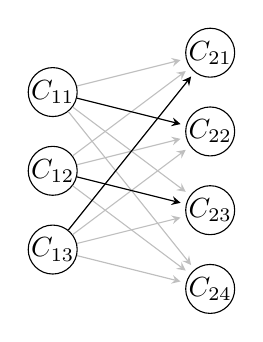
\begin{tikzpicture}[
    >=stealth,
    clus/.style={circle,draw=black,inner sep=0,minimum size=5mm},
    dist/.style={->,shorten >=2pt},
    faint/.style={dist,gray!50},
    match/.style={dist,black}
    ]

    \node [clus] (c11) at (0,1) {$C_{11}$};
    \node [clus] (c12) at (0,0) {$C_{12}$};
    \node [clus] (c13) at (0,-1) {$C_{13}$};

    \node [clus] (c21) at (2,1.5) {$C_{21}$};
    \node [clus] (c22) at (2,.5) {$C_{22}$};
    \node [clus] (c23) at (2,-.5) {$C_{23}$};
    \node [clus] (c24) at (2,-1.5) {$C_{24}$};

    % join them all
    \foreach \x in {1,2,3} {
      \foreach \y in {1,2,3,4} {
        \draw [faint] (c1\x) to (c2\y);
      }
    }

    % matches
    \draw [match] (c11) to (c22);
    \draw [match] (c12) to (c23);
    \draw [match] (c13) to (c21);
  \end{tikzpicture}
  \caption{An injection, $\sigma$, is sought among all possible injections
    $\sigma \colon \{1,\dotsc,k\} \to \{1,\dotsc,k'\}$ where $k' \geq k$.
    This is used to ``match'' pairs of clusters.}
  \label{fig:matching}
\end{figure}

The first is a similarity measure due to \citet{meila-2001} that finds a
match for $k$ clusters using a heuristic: the greatest value in the confusion
matrix, $n_{ab}$ say, gives us the first match---between clusters $C_{1a}$ and
$C_{2b}$.  The next match is then given by the greatest value not in row $a$
or column $b$, and so on until $k$ matches are found.  Thus we find an
injection, $\sigma \colon \{1,\dotsc,k\} \to \{1,\dotsc,k'\}$.  This is
illustrated in Figure~\ref{fig:matching}.  Given an injection, $\sigma$, found
as described, the measure is then:
\begin{equation*}
  \partcompare{H} = \frac{1}{n} \sum_{i=1}^{k} n_{i \sigma(i)}.
\end{equation*}

A second similarity measure, introduce by \citet{larsen-aone-1999}, makes
locally maximal matchings for each cluster:
\begin{equation*}
  \partcompare{L} = \frac{1}{k} \sum_{i=1}^{k} \max_{1 \leq j \leq k'}
                                             \frac{2n_{ij}}{|C_{1i}|+|C_{2j}|}.
\end{equation*}

A dissimilarity measure, which is a metric, was introduced by
\citet{van-dongen-2000}.  This measure computes two matching functions and,
again, makes locally maximal matchings:
\begin{equation*}
  \partcompare{V} = 2n - \sum_{i=1}^{k} \max_{1 \leq j \leq k'} n_{ij}
                         \sum_{j=1}^{k'} \max_{1 \leq i \leq k} n_{ij}.
\end{equation*}

A second metric is due to \citet{meila-2005} and is know as
\textit{classification error}.  Here, a globally maximal injection $\sigma
\colon \{1,\dotsc,k\} \to \{1,\dotsc,k'\}$ is found out of all possible
injections, $S_k$; the measure is then:
\begin{equation*}
  \partcompare{CE} = 1 - \frac{1}{n} \max_{\sigma \in S_k}
                                     \sum_{i=1}^{k} n_{i \sigma(i)}.
\end{equation*}
The injection, $\sigma$, can be found in polynomial time as the solution to a
linear program.  This metric has the additional property that it has an upper
bound of $1$.

\begin{table}
  \centering
  \begin{tabular}{lr}
    \toprule
    Name & Measure \\
    \midrule
    Meilă \& Heckerman   & $\partcompare{H} \approx 0.556$ \\
    Larsen \& Aone       & $\partcompare{L} \approx 0.622$ \\
    Van Dongen metric    & $\partcompare{V} = 7.000$ \\
    Classification Error & $\partcompare{CE} \approx 0.445$ \\
    
    \bottomrule
  \end{tabular}
  \caption{Various set matching based measures applied to $\clus_1$ and $\clus_2$.}
  \label{tab:set-matching-comparison}
\end{table}

The values of the set matching measures when applied to our example partitions
are given in Table~\ref{tab:set-matching-comparison}.

\citet{meila-2007} and \citet{bae2010comparison} point out that all of these
measures suffer from the so-called ``problem of matching'' which we will now
illustrate.  Given a partition, $\clus$, with $k$ equally sized clusters we
can obtain a second partition, $\clus'$, by moving a fraction, $f$, of the
objects from each cluster, $C_{i}$, to $C_{(i+1) \mod k}$.  We can obtain a
third partition, $\clus''$, from $\clus$ by taking the same fraction from each
cluster and distributing the objects evenly among all other clusters.  Our
intuition would be that the similarity between $\clus$ and $\clus'$ is not the
same as the similarity between $\clus$ and $\clus''$.  However,
$\partcomparep{H} = \partcomparepp{H}, \partcomparep{L}
= \partcomparepp{L}, \partcomparep{V} = \partcomparepp{V}$ and
$\partcomparep{CE} = \partcomparepp{CE}$ whenever $f < 1/2$.

To give a numerical example, let
\begin{equation*}
  \clus = \{\{1,2,3,4,5\},\{6,7,8,9,10\},\{11,12,13,14,15\}\}
\end{equation*}
and $f = 2/5$.  Our other partitions are therefore
\begin{equation*}
\clus' = \{\{1,2,3,14,15\},\{6,7,8,4,5\},\{11,12,13,9,10\}\}
\end{equation*}
and
\begin{equation*}
\clus'' = \{\{1,2,3,9,14\},\{6,7,8,4,15\},\{11,12,13,5,10\}\}.
\end{equation*}
In this case we have
\begin{align*}
  \partcomparep{H} &= \partcomparepp{H} = 3/5,\\
  \partcomparep{L} &= \partcomparepp{L} = 3/5,\\
  \partcomparep{V} &= \partcomparepp{V} = 12,\\
  \partcomparep{CE} &= \partcomparepp{CE} = 2/5.
\end{align*}


\subsubsection{Information theoretic}
\label{sec:inform-theor}

Two measures which use information theory are \textit{Normalized Mutual
  Information} \citep{fred-jain-2003} and \textit{Variation of Information}
\citep{meila-2007}.  We will look at the latter measure now.

Variation of Information is based on both how much information is contained in
each partition and how much information one partition contains about the other
(their mutual information).  The first part is measured by
\begin{equation*}
  H(\clus_1) = -\sum_{i=1}^{k} P_1(i) \log_b P_1(i),
\end{equation*}
where
\begin{equation*}
  P_1(i) = \frac{|C_{i1}|}{k}, \qquad \text{for $i = 1,\dotsc,k$}.
\end{equation*}
This is the probability that an object picked randomly from $\dset$ is in
cluster $C_{1i}$.  This measure is sometimes called the \textit{entropy}.  The
base of the logarithm determines the unit of information---$b=2$ gives the
information in \textit{bits}, $b=e$ gives \textit{nits} and $b=10$ gives
\textit{Hartleys} \citep{kullback68information}.

The mutual information is given by
\begin{equation*}
  I(\clus_1,\clus_2) = \sum_{i=1}^{k} \sum_{i=1}^{k'}
                      P_{12}(i,j) \log_b \frac{P_{12}(i,j)}{P_1(i)P_2(j)},
\end{equation*}
where
\begin{equation*}
  P_{12}(i,j) = \frac{|C_{1i} \cap C_{2j}|}{n}, \qquad \text{for $i =
    1,\dotsc,k,j = 1,\dotsc,k'$}.
\end{equation*}
This is the probability that an object picked randomly from $\dset$ is in
both $C_{1i}$ and $C_{2j}$.

Variation of Information, $\partcompare{VI}$, is then defined as
\begin{equation*}
  \partcompare{VI} = H(\clus_1) + H(\clus_2) - 2I(\clus_1,\clus_2).
\end{equation*}
This is a metric with some nice properties.  First is $n$-invariant, meaning
its value depends only on the relative sizes of the clusters and not on the
number of elements in $\dset$.  Secondly, it is bounded for all $n$ by
\begin{equation*}
  \partcompare{VI} \leq \log_b n.
\end{equation*}
Further, if $\max(k,k') \leq k^*$ where $k^* \leq \sqrt{n}$ then the following
bound holds
\begin{equation*}
  \partcompare{VI} \leq 2 \log_b k^*.
\end{equation*}

\begin{table}
  \centering
  \begin{tabular}{lr}
    \toprule
    Name & Measure \\
    \midrule
    Information & $H(\clus_1) \approx 1.585$ \\
                & $H(\clus_2) \approx 1.975$ \\
    Mutual information & $I(\clus_1,\clus_2) \approx 0.834$ \\
    Variation of Information & $\partcompare{VI} \approx 1.891$
    \\
    \bottomrule
  \end{tabular}
  \caption{Variation of Information and its components applied to $\clus_1$
    and $\clus_2$ using base 2 for the logarithms.}
  \label{tab:vi-comparison}
\end{table}

The values of Variation of Information and its components applied to our
example partitions are given in Table~\ref{tab:vi-comparison}.

\subsubsection{Density based}
\label{sec:density-based}

The last category contains a metric called \textit{ADCO} which we will
describe briefly.  None of the measures so far take into account the values of
the data contained within the objects.  ADCO assumes that the data are
real-valued vectors and uses the components of the vectors to calculate
distances \citep{bae2010comparison}.  The problem with ignoring distances is
discussed, and a new solution given, in Chapter~\ref{cha:assignment-metric}.

\section{Partional clustering}
\label{sec:part-clust-algor}

The problem of finding meaningful partitions of a dataset is called
partitional clustering.  In the following subjection we will discuss the
motivation for clustering and just a few of its many applications.  Then we
will discuss the problem itself which is broadly divided into two parts: first
one must decide what a meaningful partition actually is, and for this many
criteria have been suggested, and then one can attempt to find a good
partition according to that criterion.

\subsection{Motivation}
\label{sec:part-clus-motivation}

Broadly speaking, the applications of partitional clustering fall into two
categories: data reduction and object classification.

Data reduction may be desirable when a dataset is large and it is deemed that
only an essence of the data is necessary for the statistical precision
required.  If the data is to be displayed graphically to a user then an
overwhelmingly large dataset may not be desirable.  One real-world application
of data reduction in the latter category is the display of geographical data
on an electronic map.  By applying clustering, nearby elements can be grouped
to reduce clutter on the map.

Object classification finds applications in many fields including the natural
sciences, marketing and economics, computer science and engineering.  Given a
dataset obtained by market research one may wish to find different classes of
consumers in order to observe their habits and predict future behaviour.
Document clustering is an important area concerned with clustering on datasets
consisting of objects written in a natural language.  Search engines such as
those found on the World Wide Web use clustering to suggest ``similar''
documents to the one the user is currently interested in, amongst other things
\citep{steinbach2000comparison}.

\subsection{Criteria}
\label{sec:criteria}

Informally, a good partition of a dataset is one where the clusters are
homogeneous---meaning objects belonging to the same cluster are similar---and
well-separated---meaning objects belonging to different clusters are
dissimilar.

The task of judging a particular cluster based on these informal standards is
often a highly subjective one but, nevertheless, many objective criteria have
been devised for the purposes of automatic clustering.  It is the job of a
partitional clustering algorithm to find the globally optimal solution, which
means either the minimum or maximum according to a particular criterion.

We begin with a non-exhaustive list (from \citep{hansen1997mathprog}) of the
most general of criteria---those which only require a matrix if
dissimilarities between pairs of elements to compute them.  Let $\dset =
\{x_1,x_2,\dotsc,x_n\}$ be a dataset, $\clus = \{C_1,C_2,\dotsc,C_k\}$ be a
partition of $\dset$ and $d$ a dissimilarity measure on the elements of
$\dset$.  For the following criteria we do not need to know the values of the
elements of $\dset$, or how $d$ is computed, we only need the $n \times n$
dissimilarity matrix constructed by $d$.

The following criteria measure the homogeneity of a particular cluster, $C_i$.
The \textit{diameter} is the maximum dissimilarity between two members of the
cluster:
\begin{equation*}
  \max_{x,y \in C_i} d(x,y).
\end{equation*}
The \textit{radius} is the minimum of the maximum dissimilarities between each
member and another member of the cluster:
\begin{equation*}
  \min_{x \in C_i} \max_{y \in C_i} d(x,y).
\end{equation*}
The \textit{star} is the minimum of the sums of dissimilarities between each
member and every other member of the cluster:
\begin{equation*}
  \min_{c \in C_i} \sum_{x \in C_i} d(x,c).
\end{equation*}
The \textit{clique} is the sum of dissimilarities between each pair of members
of the cluster:
\begin{equation*}
  \sum_{x,y \in C_i} d(x,y).
\end{equation*}

The following criteria measure the separation of a cluster, $C_i$, from every
other cluster.  The \textit{split} is the minimum dissimilarity between a
member of the cluster and an element outside of the cluster:
\begin{equation*}
  \min_{x \in C_i, y \in \dset \setminus C_i} d(x,y).
\end{equation*}
The \textit{cut} is the sum of dissimilarities between all members of the
cluster and all elements outside of the cluster:
\begin{equation*}
  \sum_{x \in C_i} \sum_{y \in \dset \setminus C_i} d(x,y).
\end{equation*}

Criteria for whole partitions could then be simply the sum over all partitions
of one of these criteria.  We call them \textit{sum-of-diameters},
\textit{sum-of-radii}, \textit{sum-of-stars} and so on.  Alternatively one
could simply take the maximum or minimum value, as appropriate, over the
clusters which we would call \textit{max-diameter}, \textit{max-radius},
\textit{min-cut} and so on.  Clearly one would wish to minimise the criteria
for homogeneity and maximise those for separation.

Some criteria for homogeneity are equivalent to criteria for separation.  Most
notably, minimising sum-of-cliques is equivalent to maximising sum-of-cuts.
Such a criterion is therefore a criterion for both homogeneity and separation.

Those criteria which only measure one or the other, like min-split and
max-diameter, are often conflicting.  For example, maximising min-split
produces in clusters with poor homogeneity, called the chaining effect, and
minimising max-diameter results in clusters with poor separation, called the
dissection effect.  Such criteria are therefore not so useful on their own,
but one could consider a criterion for homogeneity and a criterion for
separation simultaneously.  This is called a bicriterion
\citep{delattre1980bicriterion}.

If the dataset is actually embedded in $m$-dimensional Euclidean space then
the following criteria based on the scatter or dispersion matrix of
\citet{wilks60} are possible.  The total scatter matrix for $\dset$ is a $m
\times m$ matrix defined
as:
\begin{equation*}
  \mathbf{T} = \sum_{i=1}^{n} (x_i - \bar{x})(x_i - \bar{x})^{\mathrm{T}}
\end{equation*}
where $\bar{x}$ is the mean value of $\dset$.  Two further matrices are
the within-cluster scatter matrix, $\mathbf{W} = \sum_{i=1}^{k} \mathbf{W}_i$,
where $\mathbf{W}_i$ is the scatter matrix for cluster $C_i$, and between
cluster scatter matrix
\begin{equation*}
  \mathbf{B} =
  \sum_{i=1}^{k} |C_i| (c_i - \bar{x}) (c_i - \bar{x})^{\mathrm{T}}
\end{equation*}
where $c_i$ is the mean of cluster $C_i$.  These matrices are related by the
equality
\begin{equation*}
  \mathbf{T} = \mathbf{W} + \mathbf{B}.
\end{equation*}

One possible criterion is the minimisation of the trace of $\mathbf{W}$.  This
is equivalent to minimising the trace of $\mathbf{B}$ since
\begin{equation*}
  \tr(\mathbf{T}) = \tr(\mathbf{W}) + \tr(\mathbf{B})
\end{equation*}
and $\mathbf{T}$ is a constant.  This criterion is actually equivalent to
minimising the sum over all clusters of the sum of Euclidean distances squared
between each member of the cluster and its centroid:
\begin{equation}
  \label{eq:tr(W)}
  \tr(\mathbf{W}) = \sum_{i=1}^{k} \sum_{x \in C_i} d^2(x,c_i),
\end{equation}
where $d$ is the Euclidean distance.  This can be seen easily by examining the
main diagonal of each $\mathbf{W}_i$:
\begin{multline*}
  \mathbf{W}_i = \\
  \sum_{x \in C_i}
  \begin{bmatrix}
    (x_1-c_{i1})^2 & (x_1-c_{i1})(x_2-c_{i2}) & \cdots &
    (x_1-c_{i1})(x_m-c_{im}) \\
    (x_2-c_{i2})(x_1-c_{i1}) & (x_2-c_{i2})^2 & \cdots &
    (x_2-c_{i2})(x_m-c_{im}) \\
    \vdots & \vdots & \ddots & \vdots \\
    (x_m-c_{im})(x_1-c_{i1}) & (x_m-c_{im})(x_2-c_{i2}) & \cdots &
    (x_m-c_{im})^2
  \end{bmatrix}
\end{multline*}
where $x_j$, $c_{ij}$ mean the $j$th component of $x,c_{i}$ respectively.

Similarly, maximising $\tr(\mathbf{B})$ is equivalent to maximising the sum of
Euclidean distances squares between each cluster centroid and $\bar{x}$,
multiplied by the cluster's cardinality:
\begin{equation}
  \label{eq:tr(B)}
  \tr(\mathbf{B}) = \sum_{i=1}^{k} |C_i| d^2(c_i,x).
\end{equation}
For this reason, this criterion is often called ``sum-of-squares'', although
this name is ambiguous since any criterion utilising sums of distances squared
could have this name.  We therefore call it \textit{centroid-distance}, due to
measuring the distances between elements and centroids, and in general call
any criterion using sums of distances squared a sum-of-squares criterion.
Note that when centroid-distance is calculated using
equation~\eqref{eq:tr(W)}, we can use any metric for $d$.  If it is calculated
using the scatter matrix then it is implicitly using the Euclidean metric.

The relationship between equations~\eqref{eq:tr(W)} and \eqref{eq:tr(B)} can
also be shown by the Huygens-Steiner, or parallel-axis, theorem, which states
that
\begin{equation}
  \label{eq:huygens}
  \sum_{x \in C_i} d^2(x,s) = d^2(c_i,s) \dot |C_i| + \sum_{x \in C_i} d^2(x,c_i)
\end{equation}
where $s$ and the members of $C_i$ are in Euclidean space and $d$ is the
Euclidean distance.

We can also use this theorem to show a relationship between centroid-distance
and sum-of-cliques.  Beginning with equation~\eqref{eq:huygens} we assign some
$y \in C_i$ to $s$ and sum over all $y \in C_i$:
\begin{equation*}
  \sum_{x,y \in C_i} d^2(x,y) = \sum_{y \in C_i} d^2(c_i,y) \dot |C_i|
                           + \sum_{x \in C_i} d^2(x,c_i) \dot |C_i|
\end{equation*}
and, since $d$ is symmetric,
\begin{equation}
  \label{eq:cd-as-equivalence}
  \frac{\displaystyle \sum_{x,y \in C_i} d^2(x,y)}
       {|C_i|}
  = 2 \sum_{x \in C_i} d^2(x,c_i).
\end{equation}
So when we use Euclidean distance squared as dissimilarity measure,
centroid-distance for each cluster is equivalent to sum-of-cliques over twice
the cardinality of the cluster.  Since $d$ is symmetric this is the same as
only counting pairwise distances once each.

It should be noted that centroid-distance is, in fact, simply a more general
version of sum-of-stars where the centre need not be a member of the dataset
but is a member of the underlying metric space.

As mentioned, we generally call any criterion involving a metric squared a
sum-of-squares criterion.  We call the numerator of the left-hand side of
equation~\eqref{eq:cd-as-equivalence} \textit{all-squares}, since we sum over
all pairs of distances.  Since sum-of-cliques can generally be used with any
dissimilarity measure we generally count each pair of elements twice, once in
each direction, but for a metric this is obviously redundant.

Two other criteria based on the scatter matrix, which were suggested by
\citet{friedman1967criteria}, are the minimisation of the determinant of
$\mathbf{W}$, sometimes called generalised variance, and the maximisation of
the trace of $\mathbf{BW}^{-1}$.  These criteria tend to produce clusters of
similar shape and size as centroid-distance with the Euclidean metric
\citep{marriott1982optimization}.

A further four criteria based on the scatter matrix are discussed in
\citep{marriott1982optimization}, these are
$\prod_{i=1}^{k}|\mathbf{W}_i|^{|C_i|}$, which is a generalisation of
$|\mathbf{W}|$ that allows cluster of different shapes,
$\sum_{i=1}^{k}|\mathbf{W}_i|^{\frac{1}{m}}$, introduced in
\citep{maronna1974}, $n \log{|\mathbf{W}|} - 2\sum_{i=1}^{k} |C_i|
\log{|C_i|}$ and $\sum_{i=1}^{k} (|C_i| \log{|\mathbf{W}_i|} -
2|C_i|\log{|C_i|})$.

All of the criteria based on the scatter matrix tend to produce ellipsoidal
clusters; clusters with other shapes will either not be found or be divided
into small clusters \citep{marriott1982optimization}.  Most of the criteria
also tend to produce clusters which are linearly-separable---meaning they are
separated by hyperplanes.

Some criteria are based on similarities instead of dissimilarities.  One such
example is the average entity stability of \citep{Rubin67optimal}.  This
criterion considers an object to be stable if it is more attracted to the rest
of the cluster it is currently in than to any other cluster.  Attraction to a
cluster is the average similarity between the object and the members of that
cluster.  The criterion is to maximise the average entity stability over the
whole dataset.

Criteria based on information theory are also possible.
\citet{wallace1968information} contains a clustering program called SNOB which
attempts to optimise one such information measure.

We finish our discussion on criteria with two further definitions.  The
partition which is the global minimum or maximum solution, whichever is
appropriate, for a particular criterion is called the optimal partition, for
example, we will later refer to the centroid-distance optimal partition,
all-squares optimal partition and so on.  The problem of finding an optimal
partition according to any criterion we will refer to simply as clustering,
and when we speak of a particular criterion we will say centroid-distance
clustering, all-squares clustering and so on.

\subsection{Computational complexity}
\label{sec:complexity-issues}

Given the huge space of possible partitions of a dataset, partitional
clustering is intuitively a hard problem.  In fact, it has been shown that
many partitional clustering problems are NP-complete.

A number of partitional clustering problems were shown to be in NP-complete by
\citet{brucker1978complexity}.  Among these was max-diameter clustering, a
result which is directly deducible from the earlier results of
\citet{sahni1976p}.  Max-diameter clustering remains NP-complete for $k=3$ and
when all dissimilarities are in $\{0,1\}$ \citep{gareyjohnson79}.

Sum-of-cuts (and therefore sum-of-cliques) is equivalent to the classic
NP-complete graph problem, MAX CUT
\citep{karp72twentyone,gonzalez1982computational}.  The problem is NP-complete
for $k=2$ and even when all dissimilarities are in $\{0,1\}$
\citep{garey76simplified}.  An approximate solution to sum-of-cuts is possible
to find in polynomial time, but the approximation problem of sum-of-cliques
remains NP-complete \citep{sahni1976p}.

It was shown in \citet{gonzalez1985clustering} that max-diameter clustering is
NP-complete when the dataset is in 2-dimensional Euclidean space and the
Euclidean metric is used.  It is also shown that for a general dissimilarity
function, even finding an approximate solution to within some known degree of
the optimal is NP-complete.

For a dataset in 1-dimensional Euclidean space the problem is solvable in
polynomial time.  Further, whenever the dissimilarity measure satisfies the
triangle inequality it possible to find an approximate solution efficiently.
\citet{brucker1978complexity} provides an algorithm for finding solutions with
a max-diameter within two times the max-diameter of the optimal solution.

\citet{bern1996approximation} show that, under the Euclidean metric, it is
NP-complete to find approximate solutions with a max-diameter within 1.969
times the max-diameter of the optimal, and with a max-radius within 1.822
times the max-radius of the optimal.

Another result of \citet{brucker1978complexity} is that sum-of-diameters
clustering is NP-complete for $k \geq 3$.  \citet{doddi2000approximation} show
that approximate solutions with a sum-of-diameters within two times the
optimal can be found efficiently, but only when the dissimilarity satisfies
the triangle inequality.  If the triangle inequality is not satisfied then it
shown that, if $P \neq NP$, no efficient approximation algorithm is possible,
even for $k=3$.

In \citet{hansen87sumofdiameters} it is shown that the problem when $k=2$ is
solvable in $O(n^2 \log n)$ time.  It is also shown that minimising any
function of the diameters can be done in $O(n^5)$ time when $k=2$.

In \citet{garey82quant} it is shown that the quantization problem is
NP-complete for $k \geq 2$.  This problem is stated as follows:

\begin{quote}
  A source produces one sample of a random variable $X$ with equiprobable
  values in $\{1,2,\dotsc,n\}$.  The encoder (quantizer) maps $X$ into a
  variable $Y$ with values in $\{1,2,\dotsc,k\}$. The decoder maps $Y$ into a
  decision variable $Z$ with values in $\{1,2,\dotsc,m\}$. If $X = i$ and $Z =
  j$ the resulting distortion is $d_{ij}$.  All entries in the $n \times m$
  matrix $[d_{ij}]$ are zeros or ones. The goal is to find an encoder
  function, $f \colon X \to Y$, and a decoder function, $g \colon Y \to Z$,
  such that the average distortion
  \begin{equation*}
    \frac{1}{n} \sum_{i=1}^{n} d_{ig(f(i))}
  \end{equation*}
  is as small as possible.
\end{quote}

It it easy to see that this problem is equivalent to a specific case of
sum-of-stars clustering where all dissimilarities are in $\{0,1\}$.

The above complexity results, especially the last one for sum-of-stars, has
led many authors to believe that centroid-distance clustering in Euclidean
space is also NP-complete.  In fact this was proved only relatively recently.
It is in fact NP-complete even when $k=2$ \citep{aloise09exact} and for
general $k$ in 2-dimensional Euclidean space \citep{mahajan09}.  If both $k$
and $s$, the number of dimensions, are fixed, then the problem is exactly
solvable in $O(n^{sk+1} \log n)$ time \citep{inaba94weightedvoronoi}.

Not all criteria are hard to optimise.  Min-split is one criterion for which
optimal clusterings can be found efficiently.  This can be done using the
single-link hierarchical clustering algorithm of
\citet{johnson67hierarchical}.  The runtime of this algorithm is $O(n^2)$
\citep{delattre1980bicriterion}.  However, this criterion does suffer from the
previously mentioned chaining effect and for this reason it is often paired
with a criterion for homogeneity in a bicriterion.  It is unlikely that any
criteria exist which produce good solutions and can be optimised efficiently.

\subsection{Methods}
\label{sec:methods}

The consequence of the complexity issues discussed in the previous section are
that heuristic methods for approximating optimal solutions are very
prevalent.  There are only a small handful of algorithms which are either
guaranteed to find a globally optimal solution or guaranteed to find a
solution within a known degree of the optimal.

Many of the heuristic algorithms happen in two stages:
\begin{enumerate}
\item \label{item:initpart} Select some initial partition,
\item \label{item:improvepart} Try to improve the partition with respect to
  some criterion.
\end{enumerate}
We will first look at some methods for stage~\ref{item:initpart}.

A common way to select an initial partition is to choose $k$ elements to be
initial estimates for the ``centre'' of each cluster.  The elements of the
dataset are then grouped with the centre that is closest.  Sometimes the
centres are updated each time a new element is grouped with them, for example
they could become the actual centroid or medoid of that cluster.  The $k$
centres are usually selected from the dataset, but they could also be taken
from the underlying metric space.

Some simple ways to select $k$ centres are to take the first $k$ elements of
the dataset \citep{macqueen1967some}, $k$ random elements of the dataset
\citep{forgy65cluster} or $k$ elements regularly spaced across the dataset
\citep{beale1969euclidean}.

The Kennard-Stone algorithm (Algorithm~\ref{alg:kennard-stone}) finds $k$
centres that are maximally separated in the metric space.

\begin{algorithm}
  \caption{Kennard-Stone initial centres algorithm.}
  \label{alg:kennard-stone}

  \begin{algorithmic}
    \Require Number of centres desired, $k \geq 2$, and a dataset, $\dset =
             \{x_1,x_2,\dotsc,x_n\}$ with $n \geq k$, with distance function
             $d \colon \dset \times \dset \to \mathbb{R}^+$.
    \Ensure Centres $\{c_1,c_2,\dotsc,c_k\} \subseteq \dset$.

    \State $\displaystyle (c_1,c_2) \gets
            \argmax_{(c,c') \in \dset \times \dset} d(c,c')$
    \State $S \gets \{c_1,c_2\}$
    \State $m \gets 2$

    \While{$m < k$}
       \State $\displaystyle c_{m+1} \gets
               \argmax_{c \in \dset \setminus C}
               \min_{\raisebox{-.2em}{$\scriptstyle c' \in C$}} d(c,c')$
       \State $S \gets S \cup \{c_{m+1}\}$
       \State $m \gets m+1$
    \EndWhile

    \State \Return $S$.
  \end{algorithmic}
\end{algorithm}

It is noted by \citet{degroot1999selecting} that this method is sensitive to
outliers and it is suggested that the initial two elements are not necessarily
maximally separated; they should be distant, but not outliers.

Another method is due to \citet{yuan04initial}
(Algorithm~\ref{alg:yuan-meng}).  The authors suggest a value of 0.75 for the
parameter $\alpha$.

\begin{algorithm}
  \caption{Yuan-Meng-Zhang-Dong initial centres algorithm.}
  \label{alg:yuan-meng}

  \begin{algorithmic}
    \Require Number of centres desired, $k > 0$, $0 < \alpha \leq 1$, and a
             dataset $\dset = \{x_1,x_2,\dotsc,c_k\}$, with $n \geq k$,
             embedded in a metric space $(M,d)$.
    \Ensure Centres $\{c_1,c_2,\dotsc,c_k\} \subseteq \dset$.

    \State $m \gets 1$
    \While{$m<k$}
       \State $\displaystyle (x_i,x_j) \gets
               \argmin_{(x,x') \in \dset \times \dset} d(x,x')$
       \State $C_m \gets \{x_i,x_j\}$
       \State $\dset \gets \dset \setminus \{x_i,x_j\}$
       \While{$\displaystyle |C_m| < \alpha \cdot \frac{n}{k}$}
          \State $\displaystyle x_i \gets
                  \argmin_{x \in \dset} \min_{x' \in C_m} d(x,x')$
          \State $C_m \gets C_m \cup \{x_i\}$
          \State $\dset \gets \dset \setminus \{x_i\}$
       \EndWhile
    \EndWhile

    \ForAll{$1 \leq i \leq k$}
       \State $\displaystyle c_i \gets
               \argmin_{c \in M} \sum_{x \in C_i} d^2(x,c)$
    \EndFor

    \State \Return $\{c_1,c_2,\dotsc,c_k\}$.
  \end{algorithmic}
\end{algorithm}

A further method which is commonly used prior to either Lloyd's or Hartigan's
method for centroid-distance is called $k$-means++
(Algorithm~\ref{alg:kmeans++}).

\begin{algorithm}
  \caption{$k$-means++ initial centres algorithm.}
  \label{alg:kmeans++}

  \begin{algorithmic}
    \Require Number of centres desired, $k > 0$, dataset $\dset =
             \{x_1,x_2,\dotsc,x_n\}$, with $n \geq k$, and distance function
             $d \colon \dset \times \dset \to \mathbb{R}^+$.
    \Ensure Centres $\{c_1,c_2,\dotsc,\c_k\}$.

    \State $S \gets \{\text{element chosen at random from $\dset$}\}$
    \State $m \gets 2$
    \While{$m < k$}
       \State $\displaystyle S \gets S \cup
               \left\{\text{an element $x' \in \dset$ chosen with probability
                            $\frac{\displaystyle \min_{c \in S} d^2(x',c)}
                             {\displaystyle
                              \sum_{x \in \dset} \min_{c \in S} d^2(x,c)}$
                            }\right\}$
    \EndWhile

    \State \Return $S$.
  \end{algorithmic}
\end{algorithm}

Many other methods have been suggested and examples can be found in
\citep{he2004initialization}, \citep{khan2004clusterecenter},
\citep{cao09initialization}, \citep{yedla2010enhancing},
\citep{zhang2009initialcenters}, \citep{Erisoglu2011intiailcenters} and
\citep{redmond2007method}.

Given an initial partition there are then many different ways to improve upon
it for stage~\ref{item:improvepart}.  Some methods take a criterion as a
parameter while others are specialised for a particular criterion.

One of the oldest and simplest heuristics is due to
\citet{hartigan1975clustering}:  Given some initial partition and a criterion,
repeatedly select objects and optimally reassign them until no further
reassignments will improve make an improvement with respect to the criterion.
Clearly when termination occurs a local optimum has been found.  Many of the
earliest clustering methods simply consisted of a particular initialisation
step followed by Hartigan's method with respect to a particular criterion
\citep{everitt80}.

LLoyd's method, which is designed to optimise centroid-distance in Euclidean
space, is probably the most well-known and widely used clustering algorithm
today.  The centroid-distance problem is also commonly called $k$-means.  The
popularity of Lloyd's algorithm has led to many authors referring to it simply
as ``the $k$-means algorithm''.  There is some confusion here, though, as some
authors also refer to Hartigan's method with respect to centroid-distance as
$k$-means and others call Lloyd's method H-means.  To avoid ambiguity we avoid
any of these alternative names.

The algorithm is easy to understand and proceeds as follows:
\begin{enumerate}
\item find $k$ initial centres using a method above,
\item \label{item:lloyds-2} Assign each element to the group with the closest
  centre,
\item \label{item:lloyds-3} Set each centre equal to the centroid of the
  cluster,
\item \label{item:lloyds-4} Repeat steps~\ref{item:lloyds-2} and
  \ref{item:lloyds-3} until no new reassignments take place.
\end{enumerate}

The version written here is as suggested by \citet{ballhall67clustering}.
\citet{macqueen1967some} prefers a variation which combines
steps~\ref{item:lloyds-2} and \ref{item:lloyds-3}: the cluster centres are
updated to the new centroid each time a new elements are added or removed from
a cluster.  Usually, to enable quicker termination, another stopping condition
is added to step~\ref{item:lloyds-4}, for example a maximum number of
iterations or a minimum threshold for the changes made after each iteration.

The major advantage of LLoyd's method is that it is simple and easy to
implement (assuming centroids are easy to computer) and it is generally very
fast to converge to a local optimum.  There are many disadvantages, however.
As mentioned already, it is implicitly assumed that centroids are easy to
compute.  This is true when the dataset is embedded in Euclidean space and the
distance used is a Bregman divergence, such as Euclidean distance squared as
in the sum-of-squares centroid-distance, since the centroid is simply the mean
\citep{telgarsky2010hartigan,banerjee2005clustering}.  This is not generally
the case, though.  Calculating means does require that we have access to the
database itself rather than simply a matrix of dissimilarities, this is a
disadvantage in many applications.  A further disadvantage is that the
algorithm actually requires, in the worse case, exponentially many iterations
to converge, even in the plane \citep{vattani2009exponential}.

Despite these drawbacks, Lloyd's method remains very popular.  In a brief
survey of some popular data mining and machine learning software it was found
that Lloyd's method is used in around three-quarters of implementations for
centroid-distance clustering.  Hartigan's method is used the rest of the time
including in some of the more prominent software, for example in Weka and R.
A comparison of Lloyd's method and Hartigan's method, in which Hartigan's
method is shown to be slightly better, is given in
\citep{telgarsky2010hartigan}.

Sum-of-stars clustering is also known as $k$-medoids clustering.  The oldest
and simplest heuristic for sum-of-stars is Partitioning Around Medoids (PAM)
as introduced in \citet{kaufman2005finding}.  The algorithm proceeds as
follows:
\begin{algorithm}
  \caption{PAM}
  \begin{enumerate}
  \item Initialise a partition $\{C_1,\dotsc,C_k\}$ by selecting $k$ elements
    at random from $\dset$ and placing one in each cluster.  Call the set of
    $k$ selected elements $\dset_s$ and the unselected elements $\dset_u$.
  \item Assign each element in $\dset_u$ to the cluster containing the closest
    element of $\dset_s$.  Calculate the sum-of-stars for this partition.
  \item Repeatedly swap elements of $\dset_s$ with elements of $\dset_u$, and
    reassign the elements of $\dset_u$, whenever the swap would improve the
    sum-of-stars.  Continue to swap until no swap will improve the
    sum-of-stars.
  \end{enumerate}
\end{algorithm}

Since PAM requires the sum-of-stars to be calculated a potentially very large
number of times, \citet{kaufman2005finding} suggested a version with enhanced
performance for large datasets called CLARA (CLustering LArge Applications).
The basic idea is to run PAM on a subset of the dataset which is selected at
random.  The centres found by PAM in the subset should be a good approximation
for the centres that would be found by PAM in the entire dataset.  After the
centres are found in the subset, the rest of the dataset is assigned to the
cluster with the closest centre.  Usually multiple samples are taken and the
partition with the smallest sum-of-stars is taken.  \citet{kaufman2005finding}
suggest taking five samples of size $40+2k$.

Compared with PAM, CLARA performs well for larger datasets.  Each iteration of
PAM has runtime complexity of $O(k(n-k)^2)$ while for CLARA it is only
$O(k(40+k)^2 + k(n-k))$ with the suggested sample size \citep{ng2002clarans}.

CLARANS (Clustering Large Applications based on RANdomized Search) takes
influence from both PAM and CLARA \citep{ng2002clarans}.  The algorithm
considers the graph $G_{nk}$ with vertices $\{\{m_1,m_2,\dotsc,m_k\} |
m_1,m_2,\dotsc,m_k \in \dset\}$---all possible $k$-medoids, which each define
a partition.  Two vertices, $M_1$ and $M_2$ are connected by an edge if and
only if $|M_1 \cap M_2| = k-1$---they differ by only one object.

PAM can be thought of as a search through this graph to find a vertex for
which no adjacent vertices have a lower sum-of-stars.  PAM considers every
adjacent vertex at each stage in the search.  CLARA instead searches through
only a subgraph which is much smaller than $G_{nk}$ so does not consider every
adjacent vertex at each stage.

CLARANS searches through the entire graph $G_{nk}$, but does not check every
adjacent vertex at each step, instead if considers a random subset of the
adjacent vertices.  It proceeds as follows:
\begin{algorithm}
  \caption{CLARANS}
  \begin{enumerate}
  \item Require parameters $numlocal$ and $maxneighbour$.  Set $i \gets 1$ and
    $mincost$ to a large number,
  \item Set $current$ to a random vertex of $G_{nk}$,
  \item Set $j \gets 1$,
  \item Compare the sum-of-stars of $current$ and a random vertex, $S$,
    adjacent to $current$,

    If $S$ has a lower cost, set $current \gets S$ and go to 3,

    Otherwise, set $j \gets j+1$,
  \item If $j \leq maxneighbour$, go to 4,

    Otherwise, if $ss(current)<mincost$, set $mincost \gets ss(current)$ and
    $bestnode \gets current$,
  \item Set $i \gets i+1$m

    If $i \leq numlocal$, go to 2,
  
    Otherwise return $bestnode$.
  \end{enumerate}
\end{algorithm}

In experiments, CLARANS was shown to run faster than PAM while producing
higher quality output than CLARA \citep{ng2002clarans}.

Heuristics remain the most popular choice for clustering applications in
general, probably due to their ability to produce acceptable solutions for a
wide variety of input.  But it is often more desirable to have a proper
algorithm; one with a proven worst-case runtime complexity and which is
guaranteed to produce optimal solutions, or solutions within some known degree
of the optimal; the former type are called exact algorithms and the latter
approximation algorithms.

Approximation algorithms are a popular way to deal with many NP-hard
optimisation problems.  An algorithm is called an $n$-approximation algorithm
if the solutions produced are guaranteed to have a cost, with respect to the
objective criterion function, of no more than $n$ times (a minimisation
problem) or $1/n$ times (a maximisation problem) the cost of the optimal
solution.

\citet{gonzalez1985clustering} provides a 2-approximation algorithm for
max-diameter which has worst-case runtime complexity of $O(nk)$.  The
algorithm requires that the dissimilarity used satisfies the triangle
inequality.  \citet{doddi2000approximation} provide a 2-approximate algorithm
for sum-of-diameters which, again, requires the dissimilarity to satisfy the
triangle inequality.  They also provide a version which produces partitions of
no more than $O(k)$ clusters that has sum-of-diameters within $O(\ln(n/k))$
times the optimal for a $k$-partition.  Other approximation algorithms have
been devised for amx-radius \citep{wirth04approx} and centroid-distance
\citep{cormode2008approximation}.

Some work has been done on exact algorithms for certain criteria.  For those
problems which are NP-complete, these algorithms are only efficient under very
constrained input conditions.  Algorithms for centroid-distance exist
including methods using brand-and-bound \citep{brusco2006repetitive},
branch-and-cut \citep{aloise09exact} and column generation
\citep{merle1999interior}.  Some of these algorithms are able to find exact
solutions to instance in the plane with up to 2000 objects, in reasonable time
\citep{aloise09exact}.

The all-squares problem, or more generally sum-of-cliques, has received
attention also.  An exact algorithm using branch-and-bound
\citep{klein1991optimal} can be used to solve problems with $n \leq 50, k \leq
5$ in reasonable time \citep{hansen1997mathprog}.  Cutting planes have also
been applied with problems with $n \leq 158$ solved quickly
\citep{hansen1997mathprog,palubeckis1997branch}.

In \citet{hansen1978complete} an exact algorithm using graph-colouring for the
max-diameter problem is given which is shown to exactly cluster 270 objects in
reasonable time.

Not many clustering problems are in $P$, but one problem which has already
been mentioned is min-split which can be exactly solved using the SLINK
algorithm \citep{johnson67hierarchical,sibson1973slink}.  This is actually a
hierarchical clustering algorithm, but can be used to find partitions simply
by taking the layer of the hierarchy with the desired number of clusters.

\section{Hierarchies}
\label{sec:hierarchies}



\chapter{The Assignment Metric}
\label{cha:assignment-metric}

\section{Summary}
\label{sec:asgn-met-summary}

In this chapter we present the assignment metric and show how it can be used
as a metric on subsets in a metric space as well as partitions.

\chapter{Sum-of-Squares Clustering}
\label{cha:sum-squar-clust}

\section{Summary}
\label{sec:summary-sum-squar}

In this chapter we examine two sum-of-squares criteria for clustering in a
metric space and compare their performance.

\chapter{Tree Stuff}
\label{cha:tree-stuff}



\chapter{Further Work}
\label{cha:further-work}



\bibliographystyle{plainnat}
\bibliography{../metrics.bib,../comp-clustering.bib,../clustering.bib}

\end{document}
